\documentclass[doublespacing]{report} %,doublespacing
\usepackage{graphicx}
\usepackage{tocbibind}
\usepackage{hyperref}
\usepackage{amsmath}
\usepackage{graphicx}
\usepackage{array}
\usepackage{booktabs}
\usepackage{geometry}
\usepackage{float}
\usepackage{amsfonts}
\usepackage{lmodern}
\usepackage{setspace}
\begin{document}

\pagenumbering{gobble} % No page numbers 
\begin{titlepage}
\centering
   % \vspace{0.2cm}
    \Large\textbf{KWAME NKRUMAH UNIVERSITY OF SCIENCE AND TECHNOLOGY}
    
    %\Huge\textbf{(KNUST)}
    %\vspace{0.2cm}
      %\vspace{0.2cm}
  % \large{DEPARTMENT OF STATISTICS AND ACTUARIAL SCIENCE}
    %\vspace{0.2cm}
    
     \begin{center}

\includegraphics[width=0.5\textwidth]{logo.png}\end{center}

    \large{\textbf{Decoding Student Retention and Churn of
Vodafone (Telecel) in Kwame Nkrumah University
of Science and Technology (KNUST) }}
%\vspace{0.2cm}
   \\
   \large{\textbf{A Survival Analysis Approach}}
    \vspace{0.3cm}
    
\large{Musah Faridu Oubda

Kassim Asana

Sarpong Linda

Torsi Edmond Collins

Asiamah Ezekiel}

    \vspace{0.4cm}  
    \small{A THESIS SUBMITTED TO THE DEPARTMENT OF STATISTICS AND ACTUARIAL SCIENCE, KWAME NKRUMAH UNIVERSITY OF SCIENCE AND TECHNOLOGY IN FULFILLMENT OF THE REQUIREMENT FOR THE AWARD OF THE DEGREE OF BACHELOR OF SCIENCE IN ACTUARIAL SCIENCE}\\


\end{titlepage}

% Start numbering with Roman numerals for the Declaration
\pagenumbering{roman}
\chapter*{Declaration}

\vspace{1cm}

I hereby declare that this submission is my work towards the award of the undergraduate degree and that, to the best of my knowledge, it contains no material previously published by another person nor material that had been accepted for the award of any other degree of the university, except where due acknowledgment had been made in the text.

\vspace{2cm}

\begin{tabbing}
    \hspace{6cm} \= \hspace{4cm} \= \hspace{5cm} \kill
    \textbf{Musah Faridu Oubda} \> \makebox[4cm]{\dotfill} \> \makebox[4cm]{\dotfill} \\
    \textit{Student} \> \textit{Signature} \> \textit{Date} \\[1.5cm]
    \textbf{Kassim Asana} \> \makebox[3cm]{\dotfill} \> \makebox[3cm]{\dotfill} \\
    \textit{Student} \> \textit{Signature} \> \textit{Date} \\[1.5cm]
    \textbf{Sarpong Linda} \> \makebox[3cm]{\dotfill} \> \makebox[3cm]{\dotfill} \\
    \textit{Student} \> \textit{Signature} \> \textit{Date} \\[1.5cm]
    \textbf{Torsi Edmond Collins} \> \makebox[3cm]{\dotfill} \> \makebox[3cm]{\dotfill} \\
    \textit{Student} \> \textit{Signature} \> \textit{Date} \\[1.5cm]
    \textbf{Asiamah Ezekiel} \> \makebox[3cm]{\dotfill} \> \makebox[3cm]{\dotfill} \\
    \textit{Student} \> \textit{Signature} \> \textit{Date} \\[1.5cm]
\end{tabbing}
This thesis has been submitted and we as university supervisors affirm our approval of
its submission.\\


\begin{tabbing}
 \hspace{6cm} \= \hspace{4cm} \= \hspace{5cm} \kill
     \textbf{Certified by:}\\ 
    \textbf{Miss Sandra Addai-Henne} \> \makebox[3cm]{\dotfill} \> \makebox[3cm]{\dotfill} \\
    \textit{Supervisor} \> \textit{Signature} \> \textit{Date} \\[1.5cm]
    \textbf{Certified by:}\\ 
\textbf{Prof. Gabriel Asare Okyere } \> \makebox[3cm]{\dotfill} \> \makebox[3cm]{\dotfill} \\
    \textit{Head of Department} \> \textit{Signature} \> \textit{Date}
\end{tabbing}



 
\newpage
\chapter*{Abstract}
This study investigates student retention and churn of Vodafone (Telecel) services at Kwame Nkrumah University of Science and Technology (KNUST) using survival analysis approaches. By focusing on factors influencing student churn, the research aims to analyze patterns related to demographics and service usage. The study utilizes the Kaplan-Meier Estimator, Cox Proportional Hazards model and Accelerated Failure Time to identify at-risk students and develop strategies to enhance retention rates. The findings are intended to improve Telecel’s service offerings, enhance the student experience, and strengthen the partnership between Telecel and KNUST. This comprehensive analysis will provide valuable insights for reducing churn and improving customer satisfaction in the telecommunications sector.

\newpage
\chapter*{Dedication}
This work is dedicated to my family and friends for their unwavering support and encouragement throughout my studies. Special thanks to my advisors and colleagues who provided invaluable insights and guidance during this research.

\newpage
\chapter*{Acknowledgement}
% Acknowlege lectures and Mrs. Sandra

\newpage
\tableofcontents

\newpage
\listoffigures

\newpage
\listoftables





\newpage
\chapter{Introduction}

% Start numbering from here
\pagenumbering{arabic}

\section{Background of Study}

Ghana's telecommunications industry has experienced significant growth in recent years, with companies such as Vodafone playing a crucial role in providing mobile and internet services to people across the country \cite{bandim2022}. The industry is highly competitive, making customer retention vital for sustaining market share and profitability. Obtaining new customers is more expensive than retaining existing ones due to marketing activities, incentives, and campaigns involved. Therefore, retaining a customer is preferable to acquiring a new one. Customer churn, also known as customer attrition, refers to the loss of subscribers or customers who cease using a company’s service or product within a given period \cite{koranchirath2024}. Understanding the reasons behind customer churn helps to develop strategies to improve customer retention and help reduce churn rates in the long run.

Vodafone is one of the leading national telecommunications providers in Ghana. As of January 2020, it had over 9.3 million mobile voice subscribers, representing 13.81\% of Ghana's market share. Since becoming the majority shareholder, Vodafone Ghana has been operating the Ghana Satellite Earth Station (GSES) since 2008. GSES allows Ghana to access and utilize communications satellites orbiting the Earth for various applications, such as telephone services, internet connectivity, television broadcasting, data transmission, disaster management, and emergency communications. The operation of the earth station by Vodafone Ghana proves the company's commitment to investing in and upgrading Ghana's satellite communications capabilities.

In 2016, Vodafone partnered with Kwame Nkrumah University of Science and Technology (KNUST) to provide enhanced packages of services to the various faculties across the university's campuses to improve education services. This collaboration included telecommunications services such as SIM cards and data plans for the student and employee communities.

In February 2023, Telecel acquired 70\% shares in Vodafone, rebranding the company name to Telecel in 2024. This rebranding aimed to improve service offerings across voice and data services, money transfers, and business solutions. Telecel, founded in 1986, is an Africa-focused telecommunication company that operates primarily in Africa and converges telecommunications with fintech, e-commerce, and tech startups.

Student churn is a major issue every telecom company encounters. It leads to a loss of revenue and increases the cost of acquiring new customers. In the highly competitive telecom market, where customers have multiple service provider options, retaining customers becomes even more challenging. Companies use modern technology, computer software, and survival analysis approaches to identify at-risk students and devise strategies to enhance retention rates. This method of recognizing unsatisfied customers is known as churn prediction.

On March 14, 2024, Vodafone, along with several other telecommunications companies, was hit by outages on several underwater fiber optic cables, leading to disruptions in services, particularly internet services \cite{ghanaweb2023}. It affected about 10 countries in West Africa, including Ghana. Initially, it was estimated that the problem would be fixed within 3 days; however, this was not the case. The damage was massive, affecting the West Coast route to Europe, West Africa Cable System (WACS), and the Africa Coast to Europe (ACE), resulting in MainOne and SAT3 going offline \cite{apnews2023}. The only network that was properly functioning at the moment in Ghana was AirtelTigo (AT). To quickly prevent the loss of valuable customers to AirtelTigo, Vodafone (Telecel) took the initiative to update its customers daily on their progress and offer various bonuses to prevent customers from defecting to their competitors. This continued until the problem was fixed on April 29, 2024, when the WACS cable was repaired.

Previous studies have explored various factors that influence customer churn in a telecommunications company. This study aims to focus on the KNUST student population, uncover and analyze data gathered from students, apply survival analysis models to identify patterns related to churn (such as demographics, usage patterns, etc.), develop retention strategies, evaluate the success of these efforts, and make informed decisions.

\section{Problem Statement}

Regardless of efforts made by KNUST to partner with Telecel to provide affordable and accessible mobile communications services to the university’s populace, churn still persists. There is a lack of understanding about the factors driving student churn and retention, making it difficult to develop effective strategies to address this issue \cite{kapur2018}. This research aims to investigate the factors contributing to student churn and develop a survival analysis model for detecting at-risk students and design specific strategies to improve retention rates. It also seeks to enhance Telecel’s services, improve student experience, and foster long-term relationships between Vodafone (Telecel) and KNUST.

\section{Research Objectives}

The study aims to use survival analysis to estimate student churn rates at various levels.
%\subsection{Main Objective}
%\begin{itemize}
    %\item 
%	To develop a survival analysis techniques model to detect at-risk students to improve student retention and reduce churn of Telecel at KNUST.
%	%\end{itemize}
%	
%	\subsection{Specific Objectives}
%	\begin{itemize}
%	    \item Exploring the factors that influence student churn and retention.
%	    \item Using survival analysis models to identify students at risk of churning.
%	    \item Analyzing time-to-event data to understand the patterns and timing of student churn.
%	    \item Identifying strategies to improve retention rates and reduce churn.
%	\end{itemize}

%\section{Research Questions}
%\begin{itemize}
%    \item What factors influence student retention and churn for Telecel services at KNUST?
%    \item What is the relationship between student demographics (age, gender, year of study) and churn behavior?
%    \item How does the churn rate vary with different Telecel services (voice service, data service, internet service)?
%    \item How does the quality of Telecel network and services (coverage, internet speed) influence student retention and churn?
%    \item How can Telecel services be optimized to better meet the needs and preferences of KNUST students?
%\end{itemize}

\section{Significance of the Study}

The study offers a comprehensive understanding of the factors impacting student churn from Vodafone. This will enable the development of precise strategies to enhance retention rates, thereby minimizing churn. The study will empower KNUST to improve the telecom services offered to its students. By identifying the factors influencing student retention and churn, KNUST can work closely with Telecel to guarantee the delivery of top-notch, dependable services to its students, thereby solidifying the partnership between KNUST and Telecel. The study is all about understanding what the populace expects from Vodafone (Telecel). By knowing their specific needs and preferences, the services can be improved upon. This means improved connectivity, service plans, and less hassle from switching providers. Ultimately, it ensures a more stable and reliable service for students.

\section{Structure of the Study}

The study on student retention and churn for Telecel services at KNUST aims to investigate the factors that drive students' decisions on Telecel services usage. The study follows a structured approach.
\\Chapter one discusses the background information and the foundation for the research. The problem statement and goals are stated here.
\\Chapter two of the study contains a literature review, including several studies related to the subject at hand.
\\The third chapter focuses on the methodology and data collection techniques. There are several ways of approaching this problem, but the main focus of the study is using a survival analysis modeling tool.
\\The fourth chapter presents the models and practical application to the dataset. Detailed analysis is presented here with the aid of figures and diagrams to determine the optimal model for the research.
\\Chapter five delves into the conclusion and summarizes the results obtained. Based on the findings, recommendations are formulated.

\section{Limitation of the Study}

The limitation of this research was that the data survey only included students of KNUST who were present during the annual college elections. As a result, the coverage was limited to undergraduate students on the main campus.

\newpage
\chapter{Literature Review}


\section{Introduction}
Mobile technology has become widely used, changing how students interact, communicate, and obtain information \cite{Alqatani2020}. Student retention and churn are critical issues for universities and telecom companies alike. In the context of Vodafone's services offered to students, understanding student behavior and preferences is crucial for effective retention strategies. This project addresses this gap using survival analysis, a statistical method for examining data over time \cite{BoxSteffensmeier2020}. In this context, the event of interest is student churn, defined as the discontinuation or cessation of Vodafone SIM cards. By applying survival analysis, this project will provide valuable insights into student retention and churn factors.

\subsection{Telecommunication Industry and Customer Behavior}
The telecommunication industry is highly competitive, with customer acquisition and retention being pivotal to a company's success. Research indicates that factors such as service, pricing, customer support, and competitive offerings significantly influence customer churn \cite{Lai2021}.

\subsection{Student Retention and Telecom Services}
Students, as a demographic, exhibit unique usage patterns and service expectations. Studies show that reliable connectivity, affordable pricing, and additional benefits like educational resources influence their choice of telecom services \cite{SmithBrown2020}. For telecom companies, understanding these factors is crucial to tailoring services that meet students’ needs and enhance retention.

\subsection{History of Survival Analysis (SA)}
The origins of SA and its history spread far back to the early work on mortality by John Graunt, who published the book \textit{Natural and Political Observations on the Bills of Mortality} in 1662. The concept of “Life Tables” was introduced in this book. A new, modern era in SA started during World War II in the USA, where the reliability of military equipment was tested using SA. After World War II, SA became popular and spread to various other disciplines \cite{Jerenz2008}. The most influential papers on SA were published by Kaplan and Meier \cite{Kaplan1958} and Cox \cite{Cox1972}, in which the Kaplan-Meier product limit estimator and Cox proportional hazard model were introduced, respectively.

\subsection{Application of Survival Analysis}
Survival analysis (SA) has been successfully applied in diverse fields, including medical research, engineering (reliability analysis), finance, and economics. In finance, SA has been used to analyze a firm's vulnerability to global financial crises and identify firms at risk of failure, enabling timely interventions \cite{Lee2014, Pereira2014, Kumar2015, Iwasaki2014}. SA has also been employed to predict the optimal time to buy or sell stocks within the stock market \cite{Kumar2015}. In the banking sector, SA is utilized to assess banks' survival during financial crises, measure their strength when entering new markets \cite{Leung2010, Evrensel2008}, and conduct credit risk analysis \cite{Tsujitani2012, Baesens2005}. The widespread adoption of SA across these domains underscores its versatility and effectiveness in modeling time-to-event data and identifying the factors that influence outcomes of interest.

\section{Conceptual Review}

\subsubsection{Customer Retention and Churn}
Customer retention refers to a company's capacity or ability to maintain or retain their customer base over a specific period. High retention rates are crucial for maintaining revenue streams, reducing marketing costs associated with acquiring new customers, and fostering a positive brand reputation. Customer churn, also known as customer attrition, is the rate at which customers stop using a company's product or service. It can be caused by various factors such as dissatisfaction with the service, better offers from competitors, or changes in personal circumstances. In the telecommunications industry, market competitiveness is measured by churn rate. Telephone, internet, and mobile services are all part of telecommunications.

\section{Empirical Studies}

Imani, M. (2020) \textit{Customer Churn Prediction in Telecommunication Using Machine Learning: A Comparison Study}. The paper tackles customer churn in telecoms, emphasizing that retaining customers is cheaper than acquiring new ones. It evaluates various machine learning methods for predicting churn by comparing classifiers, target detectors, feature extraction, and feature selection techniques. The study finds that Random Forest and Feed-Forward Neural Networks with Genetic Algorithm showed high accuracy. Effective target detectors included Spectral Angle Mapper and Adaptive Subspace Detector. Clustering-Based Feature Extraction and Advanced Binary Ant Colony Optimization excelled in improving classification and feature selection. The study recommends implementing Random Forest and Neural Networks for effective churn prediction.

Melik Masarifoglu and Ali Hakan Buyuklu \textit{Applying Survival Analysis to Telecom Churn Data}. This paper emphasizes the importance of customer retention in telecoms, noting that retaining customers is more cost-effective than acquiring new ones. It employs survival analysis to estimate customer survival and hazard functions, focusing on factors like campaigns, tariffs, tenure, age, and auto-payment. The paper introduces survival analysis (SA) as a statistical method to analyze time-to-event data. It describes the Cox Proportional Hazard Model (CPHM), a widely used technique for quantifying the risk of an event occurring during the observation period. The paper uses Kaplan-Meier estimates and the Cox model to analyze the impact of various predictors on customer churn. The results show how different factors, such as campaigns and tariffs, affect customer survival probabilities. The study finds that survival analysis is effective for predicting churn and recommends its use for targeting at-risk customers and improving retention strategies.

Kavitha, V., Kumar, G. H., Kumar, S. M., \& Harish, M. (2020) \textit{Churn prediction of customer in telecom industry using machine learning algorithms}. This paper highlights the importance of customer churn in the telecommunications industry, noting its impact on revenue and customer lifetime value. It stresses the need for predictive models to identify potential churners and improve retention by enhancing service offerings. The methodology involves collecting data from Kaggle, preprocessing it by filtering and standardizing, and selecting relevant features. The prediction and classification phase uses Random Forest, Logistic Regression, and XGBoost algorithms, with each trained and tested to evaluate performance. The results reveal that Random Forest outperforms Logistic Regression and XGBoost in accuracy and performance. Visualizations, including confusion matrices and accuracy graphs, support these findings. The paper concludes by emphasizing that churn prediction is crucial for telecoms and suggests exploring lazy learning and AI techniques for future research.



\newpage
\chapter{Methodology}

\section{Introduction}

This chapter structures the research methods and procedures followed by the analysis to predict student churn of Vodafone (Telecel) in KNUST. A comprehensive explanation of the research models, mathematical formulations and interpretations are presented here. The paper compares their performance using the Concordance Index thus shedding light on their predictive capabilities.

\section{Research Design}

The study employs quantitative research. This type of research aims to establish the cause-and-effect relationships between variables. Specifically, it focuses on quantifying various aspects of students’ usage and satisfaction, rather than exploring underlying meanings or personal experiences in an open-ended manner.

\section{Pilot Survey}

Before the actual statistics were carried out, a pilot survey was held to grasp the scope of students’ understanding of the topic. It was carried out using final year students in Actuarial Science. Out of 50 questionnaires sent out, a total of 46 respondents were returned. 

\section{Data Collection}

The primary data source for this research was a survey conducted among students at Kwame Nkrumah University of Science and Technology (KNUST) in College of Science. The survey targeted students in final years (Level 400). The dataset includes a variety of questions, each capturing specific aspects relevant to the study with the aid of Google Forms.


\section{Sample Size}

The sample size of the research was determined through cluster sampling. Cluster sampling is a sampling technique in which the population is divided into groups known as clusters. A random sample is then selected from each cluster ensuring that, each cluster has an equal number of elements. It is therefore homogeneous within but heterogeneous around (clusters are different from one another but the elements within it share common factors). This sampling is employed to determine the optimal sample size as it is a robust method that allows to efficiently estimate the population by selecting entire clusters (colleges within KNUST) rather than using individual students.
\\The sample size for cluster sampling can be determined using the formula below:

\[n_0=\frac{z^2\ast p\ast\left(1-p\right)}{E^2}\]
\[n=\frac{n_0}{1+(\frac{n_0-1}{N})}\]
\[n_{cluster}=n\ \ast\ DEFF\]

Where:
\begin{itemize}
    \item \((N)\ \)is the population size.
    \item \((n_0)\) is the sample size for simple random sampling
    \item \((n)\)\ is the sample size for the population.
    \item \((n_{cluster})\) is the sample size of the clusters.
    \item \((z) \)represents the critical value.
    \item \((p)\) is the estimated proportion of the population (e.g., proportion of students with a certain behavior).
    \item \((DEFF) \) is the design effect, which accounts for the correlation among observations within the same cluster.
    \item \((E) \) is the margin of error.
\end{itemize}

Parameter Justification:

\begin{itemize}
    \item \textbf{Z-score} \((z)\): A confidence level of 95\% is chosen therefore resulting to a Z-score of 1.96.
    \item \textbf{Population}\( (N)\): The population size of KNUST students is about 85000.
    \item \textbf{Estimated Proportion \((p)\)}: To maximize sample size, we use 0.5.
    \item \textbf{Margin of Error }\((E)\): 5\% since the confidence Level is 95\%.


\end{itemize}


\[n_0\ =\frac{\left({1.96}^2\ast\ 0.5\ \ast\ 0.5\ \right)}{{0.05}^2}\]
\[n_0\approx383.82\]
\[n_0\approx384\]
\[n=\frac{384}{1+(\frac{384-1}{85000})}\]
\[n\approx384.16\]
\[n\approx384\]

\begin{itemize}
    \item \textbf{Design Effect} (\({DEFF})\): The design effect of 2 is used as the benchmark.

\end{itemize}
\[n_{cluster}=384\ \ast\ 2\]
\[n_{cluster}=768\]
\\
\\A cluster sample size of 768 students from the population of about 85000.
\\Since there are 6 clusters from which each represents the colleges, the sample size is evenly allocated across the clusters. Each cluster would have approximately 128 students.



\section{Data Pre-Processing}

In the realm of data analysis, ensuring the quality and suitability of data is paramount for deriving meaningful insights and making informed decisions. The initial phase of the study involved a thorough examination of the dataset to identify and handle missing data appropriately to ensure that subsequent analyses were conducted on a complete and representative dataset. One of the critical preprocessing tasks involved the transformation of categorical variables into numeric format. This was achieved using label encoding, a technique that assigns unique integer labels to each category with the aid of Python. The transformation restructured the dataset to facilitate survival analysis. The data was then organized to facilitate essential components such as time duration, event indicators, and relevant covariates to the variables. 

\section{Concept of Survival Analysis}

Survival analysis is a branch of statistics used to analyze time-to-event data. The primary interest lies in the time until the occurrence of the event of interest.  The time variable is usually referred to as survival time since it gives the time that an individual has survived over some follow-up period. The event is also referred to as a failure because the event of interest is usually death, disease incidence, or some other negative experience. 

\section{Censoring}

In survival analysis, not all subjects may experience the event of interest within the study period. Censoring occurs when the survival time of a subject is not fully observed. It occurs when a subject leaves the study before an event occurs, or when the study ends before the event has occurred for all subjects.


\subsection{Right-Censored}

It occurs when a subject has some loss to follow up or the study ends before the event of interest occurs. The lifetime is known to exceed a certain value meaning that, true survival time is equal to or greater than the observed survival time.

\subsection{Left-Censored}

It occurs when the event of interest has occurred before the study starts, and thus the exact survival time is known only to be less than a certain value indicating that the true survival time is less than or equal to the observed survival time.

\subsection{Interval-Censored}
It can occur if a subject’s true but unobserved survival time is within a certain known specified time interval. 
\begin{figure}[H]
    \centering
    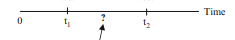
\includegraphics[width=0.4\linewidth]{Figure 3/3.1.png}
    \caption{Interval Censoring}
    \label{Figure 3.1}
\end{figure}

Interval-censoring incorporates both right-censoring and left-censoring. 

\begin{figure}[H]
    \centering
    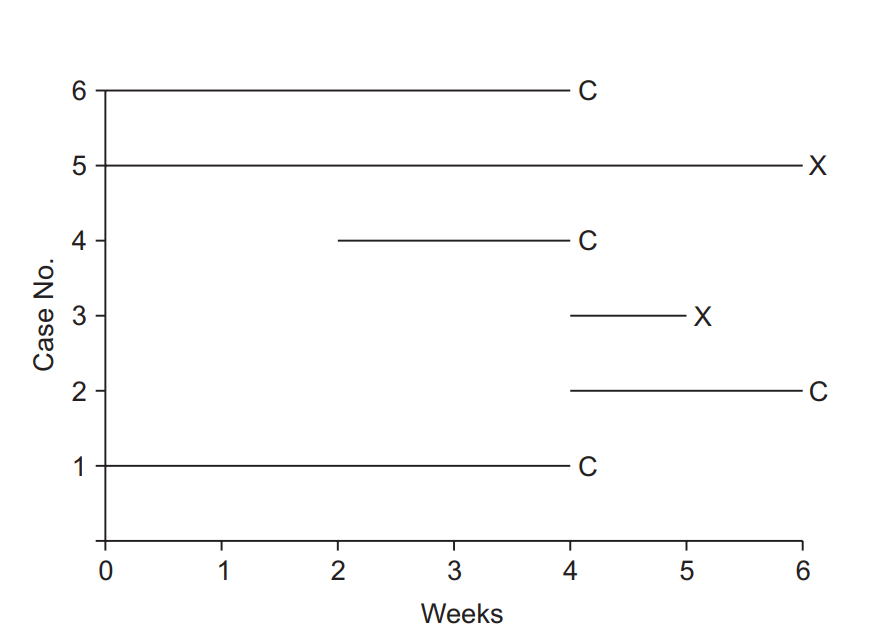
\includegraphics[width=0.5\linewidth]{Figure 3/3.2.png}
    \caption{Censoring Graph}
    \label{Figure 3.2}
\end{figure}


\begin{itemize}

\item \(C\) indicates censored data
\item  \(X\) indicates observed events


\end{itemize}


\section{Fundamental Concepts of Survival Analysis}

These functions are complementary in understanding the dynamics of survival data, namely survival function and hazard function. They are the building blocks for every survival analysis. They clearly have a defined relationship between the two. The \(S\left(t\right)\) can be derived from the \(h\left(t\right)\) complement one another such that, one can be derived from the other.

\begin{align}
\lambda(t) &= \lim_{\Delta t \to 0} \frac{\Pr(t \leq T < t + \Delta t \mid T > t)}{\Delta t} \\
&= \lim_{\Delta t \to 0} \left[ \frac{\Pr(t \leq T < t + \Delta t)}{\Delta t} \cdot \frac{\Delta t}{\Pr(T > t)} \right] \\
&= \lim_{\Delta t \to 0} \left[ \frac{\Pr(t \leq T < t + \Delta t)}{\Delta t} \right] \cdot \lim_{\Delta t \to 0} \left[ \frac{1}{\Pr(T > t)} \right] \\
&= \frac{1}{S(t)} \cdot \lim_{\Delta t \to 0} \left[ \frac{\Pr(t \leq T < t + \Delta t)}{\Delta t} \right] \\
&= \frac{1}{S(t)} \cdot \lim_{\Delta t \to 0} \left[ \frac{F(t + \Delta t) - F(t)}{\Delta t} \right] \\
&= \frac{f(t)}{S(t)}\\
S(t) &= \exp\left[-\int_{0}^{t} h(x) \, dx\right]\\
h(t) &= -\left[\frac{dS(t)/dt}{S(t)}\right]
\end{align}



The first formula describes how the survival function \(S\left(t\right)\) can be written in terms of an integral involving the hazard function. The formula states that \(S\left(t\right) \)equals the exponential of the negative integral of the hazard function \(h\left(t\right) \) between integration limits of 0 and t. 
The second formula describes how the hazard function \(h\left(t\right) \) can be written in terms of a derivative involving the survival function. The formula states that \( h\left(t\right)\) equals minus the derivative of \(S\left(t\right) \) with respect to t divided by \(S\left(t\right)\).


\subsection{\texorpdfstring{Survival Function \( S(t) \)}{Survival Function S(t)}}
The survival function \(S\left(t\right) \) also known as the survival probability function, gives the probability that a person survives longer than some specified time.

\[S(t)\ =\ P(T\ >\ t)\]
\\In equation (3), \(T\) represents the random variable for a person's survival time and \(t\) represents the specific value of interest for the random variable \(T\).
\\The survival function is  fundamental to a survival analysis as it helps in determining survival probabilities for different values of time to provide crucial summary information from the data.
\begin{figure}[H]
    \centering
    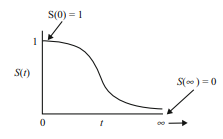
\includegraphics[width=0.45\textwidth]{Figure 3/3.31.png}
    \hfill
    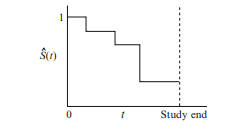
\includegraphics[width=0.45\textwidth]{Figure 3/3.32.png}
    \caption{Survivor Curves}
    \label{Figure 3.3}
\end{figure}

The figure on the left in Figure 3.3 is a theoretical curve of the survival function\ \(S\left(t\right) \) which ranges from 0 up to infinity. It is non-increasing and therefore slopes downward as \(t\) increases. At \(t= 0\), \(S\left(0\right)=1\) and when \( t\ =\ \infty , S\left(\infty\right)\ =\ 0.\) 
When actual data is used, the survivor curve does not result in a smooth curve but rather obtains a step function graph. The step function is illustrated on the right in Figure 3.3.  The study period is never infinite in duration as there may be competing risks for failure, it is possible that not everyone obtains the event of interest. The estimated survivor function \(\hat{S}\left(t\right)\), thus may not go all the way down to 0 at the end of the study.

\subsection{\texorpdfstring{Hazard Function \( h(t) \)}{Hazard Function h(t)}}

The hazard function \( h(t)\ \)denotes the instantaneous rate of failure at time \(t\), given that the subject has survived up to time\( (t).\)

\[
h(t) = \lim_{\Delta t \to 0} \frac{P(t \le T < t + \Delta t \mid T \geq t)}{\Delta t}
\]

\[h\left(t\right)\geq0\]


The hazard function \( h\left(t\right)\), is given by the formula: \(h\left(t\right)\ \)equals the limit, as \(\Delta t \) approaches zero, of a probability statement about survival, divided by \(\Delta t\), where \(\Delta t\) denotes a small interval of time.

The hazard function is also known as the conditional failure rate. It is a rate rather than a probability. In the hazard function formula, the expression to the right of the limit sign gives the ratio of two quantities. The numerator is a conditional probability while the denominator, \(\Delta t\) denotes a small-time interval. By the division, a probability per unit of time is obtained, which is no longer a probability but a rate. In particular, the scale for this ratio is not 0 to 1 like a probability but rather ranges between 0 and infinity while depending on whether time is measured in days, weeks, months, or years. 

\[H(t)=\int_{0}^{t}{h(x)dx}\]

The cumulative hazard function \(H(t)\) can be derived from the hazard function. It is the integral of the hazard function up to time \(t\). It represents the total hazard experienced up to time \( t. H(t)\) provides a straightforward cumulative measure of risk or failure over time.

\section{Approaches in Survival Analysis}

The approaches to use in survival analysis are underlined by their strengths and weaknesses. The choice is based on statistical assumptions, data characteristics and the complexity of the survival patterns to model.

\subsection{Parametric Methods}

These methods assume that the survival times follow a specific statistical distribution. Common parametric survival models are exponential, Weibull, log-normal and gamma models. They estimate parameters using maximum likelihood estimation or Bayesian methods.

\subsection{Non-Parametric Methods}

These methods include approaches that make minimal assumptions about the form of the survival distribution. Common non-parametric methods in survival analysis are the Kaplan-Meier Estimator, Nelson-Aalen Estimator and Log-Rank Test.

\subsection{Semi-Parametric Methods}

Semi-parametric models combine parametric elements (the effect of covariates) with non-parametric elements (the baseline hazard function) such as the Cox Proportional Hazard.

\section{Kaplan Meier}
The Kaplan-Meier estimator is employed in survival analysis to analyze the time until an event occurs. The Kaplan-Meier estimator calculates the survival probability at a specific time step by multiplying the probability of surviving each previous time step.
The estimator is computed as

\[S\left(t\right)=\prod_{i:t_i\le t}\left(1-\frac{d_i}{n_i}\right)\]

Where:
 \begin{itemize}
     \item \(t\) is a time
     \item \(d_i \) the number of events (churn) at time \(t_i\)
     \item \(S\left(t\right)\ \)is the survi val probability at time \(t\)
     \item \(n_i\) is the number of individuals at risk just before time \(t_i\)
 \end{itemize}
The estimator essentially calculates the probability of surviving from one time step to the next, and the product of these probabilities gives the overall survival probability up to time \(t\).

\section{Cox Proportional (Cox PH) Hazard Model}

The Cox Proportional Hazards model is a popular semi-parametric model to check the relationship between the survival time and a set of predictors.

\[
h\left(t \mid x\right) = h_0(t) \exp(\beta_1 x_1 + \beta_2 x_2 + \cdots + \beta_p x_p)
\]

Where:
 \begin{itemize}
     \item \(h(t\mid x)\) is the hazard function, i.e., the instantaneous rate of the event occurring at time \(t\) given the predictor variables \(x\).
     \item \(h_0\left(t\right)\) is the baseline hazard function, representing the hazard for individuals with all predictor variables equal to zero.
     \item \(\beta_1,\beta_2,\ldots,\beta_p\) are the coefficients for the predictor variables
 \end{itemize}

 The coefficients \(\beta\) are estimated using maximum likelihood estimation, and the model assumes a proportional hazard ratio, meaning the effect of the predictors on the hazard is constant over time.
An important assumption on the Cox PH is that it has a constant hazard function proportion for each time.


%
%                                                                \(H_0\): The Assumption of Proportional Hazard is fulfilled 
%
%                                                            \(H_1\): The Assumption of Proportional Hazard is not fulfilled 


\section{Accelerated Failure Time (AFT)}

In situations where the Cox proportional is not satisfied, the parametric model approach can be used. Accelerated Failure Time (AFT) is one of the popular parametric models used in survival analysis. The model assumes that the survival function \(S(t)\) follows a parametric continuous distribution. This implies that the distribution is following a Weibull, lognormal or exponential distribution. The aim of an AFT is to account for the influence of multiple covariates on the survival time by either accelerating or decelerating it.

\[\lambda(x)\ =\ exp(b_0\ +\ \sum_{i=1}^{n}{b_ix_i)}\]

Where:
 \begin{itemize}
     \item \(\lambda(x)\) is the accelerating factor
     \item \(b_0 \) is the baseline accelerating factor when all covariates are 0
     \item \(b_i\) is the regression coefficient
     \item \(x_i\) are the covariates

 \end{itemize}
 
\section{Akaike Information Criterion (AIC)}

The Akaike Information Criterion (AIC) is a measure of the relative quality of statistical models for a given dataset. It aids in model selection in survival analysis. It contributes by penalizing models with more parameters to avoid the problem of overfitting. The lower the AIC value, the better the model is considered to fit the data.

\[AIC=2k-2ln(L),\]

Where:
 \begin{itemize}
     \item \(k \) is the number of parameters in the model.
     \item \(L\) is the likelihood of the model
 \end{itemize}

\section{Concordance Index in Survival Analysis}

The Concordance Index, often referred to as the C-index or Harrell's C-index, is a statistical metric used to evaluate the performance of models in survival analysis. It assesses how well a model discriminates between subjects in terms of their event times and predicted risks. 

The Concordance Index measures the model's ability to correctly rank the predicted risks of individuals based on their actual event times. The Concordance Index evaluates whether the model's predicted risks align with the observed event times.

\[C=\frac{Number\ of\ Concordant\ Pairs}{Number\ of\ Concordant\ Pairs\ +Number\ of\ Discordant\ Pairs}\]

A \(C\) value above 0.5 suggests that the model has predictive ability better than random chance. A higher \(C\) value implies a better model performance and more accurate risk predictions.



\newpage
\chapter{Analysis and Findings}
\section{Introduction}

This section presents the study's findings and discusses what each output means towards the research goals. It includes easy-to-read tables, graphs, and computer results based on the methods used. The analysis closely examines details towards the model building, diagnostics and evaluation. The information here was obtained from using python for computer analysis during the research. This chapter seeks to explain the use of survival models in the methodology to determine the Vodafone (Telecel) churn rate among students.

\section{Data Description}

The dataset has a shape consisting of 768 rows and 18 columns from a sample in KNUST.

\begin{table}[H]
    \centering
    \begin{tabular}{ll}
        \toprule
        Variable & Description \\
        \midrule
        Gender & Gender of the individual (Male/Female) \\
        Churn & Whether the individual has churned (Yes/No) \\
        Residence & Type of residence (Off-campus/On-campus) \\
        Usage Frequency & Frequency of service usage  \\
        Network Strength & Strength of network (1 to 5) \\
        Voice Calls & Usage of voice calls (Yes/No) \\
        Mobile Data Internet & Usage of mobile data/internet (Yes/No) \\
        SMS Text Messaging & Usage of SMS/text messaging (Yes/No) \\
        Data Exhaustion & Whether data allowance is exhausted (Yes/No) \\
        Other Networks & Use of other networks (Yes/No) \\
        Poor Network Quality Coverage & Perception of poor network quality/coverage (Yes/No) \\
        Unsatisfactory Customer Service & Perception of unsatisfactory customer service (Yes/No) \\
        High Costs Pricing & Perception of high costs/pricing (Yes/No) \\
        Monthly Data Usage & Monthly data usage category  \\
        Churn Level & Level of churn (1 to 3 if churned, 4 if not churned) \\
        \bottomrule
    \end{tabular}
    \caption{Description of Variables}
\end{table}

\section{Model Building}

The lifelines package played a pivotal role in this section by providing essential survival analysis models in Python. These models are crucial for analyzing data where the time student churn event is important. 


\subsection{Kaplan Meier (KM) Curve}

A Kaplan-Meier curve, also known as a survival curve, is a statistical tool used in survival analysis to estimate the survival function from timeline data. It provides a way to visualize the proportion of individuals surviving over time, taking into account censored data (individuals who have not experienced the event by the end of the observation period).
\begin{figure}[H]
    \centering
    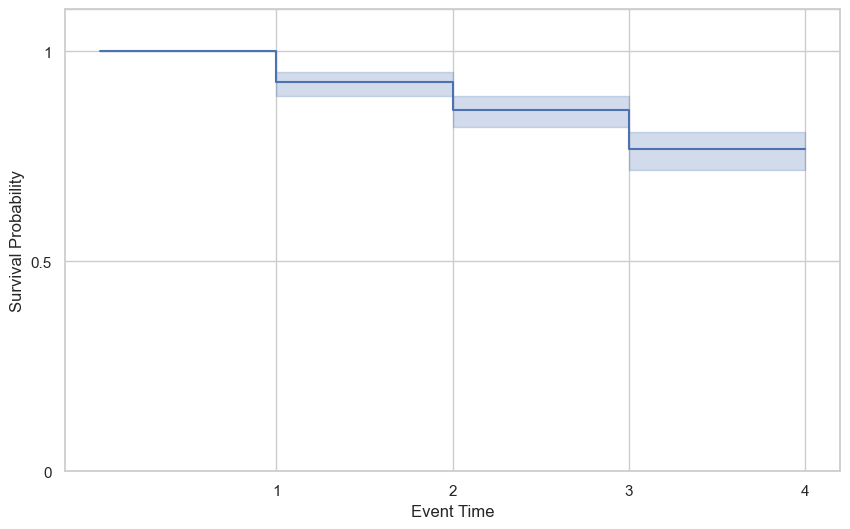
\includegraphics[width=1\linewidth]{Figure 4/4.1.png}
    \caption{Kaplan Meier Curve of students from levels 100–500}
\end{figure}

The Kaplan-Meier survival curve provided is a tool to estimate the probability that students will remain enrolled over a given time period. The x-axis represents the timeline, which in this ranges from 1 to 5 levels or years. The 0 indicates when the study began. The y-axis represents survival probability and ranges from 0 to 1.


The KM estimate line graph shows the survival probability at various points along the study. Each step down indicates an event, which decreases the overall survival probability. The shaded area around the line suggests the confidence interval, giving a range within which the true survival curve is expected to lie.

In churn prediction, this curve helps identify critical time points where student retention drops significantly and allows institutions to intervene proactively. For instance, if there’s a notable step down at a particular time point on the x-axis (3–4), it might indicate a period when students are more likely to leave and thus could be a target for retention efforts.



\subsection{Kaplan Meier Analysis}

The provided Kaplan-Meier estimator output in Table 4.2 below summarizes the survival curve in table 4.1 over level in KNUST.

\begin{table}[ht]
    \centering
    \begin{tabular}{cccccc}
        \toprule
        Event Time & Number of Individuals & Number of Events & Survival Probability & Lower CI & Upper CI \\
        \midrule
        0 & 338 & 0 & 1.000000 & 1.000000 & 1.000000 \\
        1 & 338 & 3 & 0.991124 & 0.972736 & 0.997129 \\
        2 & 335 & 6 & 0.973373 & 0.949452 & 0.986056 \\
        3 & 329 & 3 & 0.964497 & 0.938330 & 0.979681 \\
        4 & 326 & 0 & 0.964497 & 0.938330 & 0.979681 \\
        \bottomrule
    \end{tabular}
    \caption{Kaplan-Meier Survival Analysis Results}
    \label{tab:km_results}
\end{table}


Initially, at time 0 (when students initially start the academic year), all 768 students are considered to be at risk. With no events (churns) recorded yet, the survival probability is 1.
As the students ascend the academic ladder, the number at risk begins to gradually decrease as some begin to experience the event. The higher the number of events, the more the number at risk decreases. This can be seen for example, in the 2\(^{nd}\)  level where the initial 768 students from the beginning of the 1\(^{st}\) year decreased to 733 for the 2\(^{nd}\) year after 35 students churned at the end of the year. Subsequently, the survival probability declines gradually from 1 to 0.500583 by the 5\(^{th}\) year. The confidence intervals (Lower Cl and Upper CI) provide ranges within which the true survival probabilities lie with a certain level of confidence.


\subsection{Cox Proportional Hazard (COX PH)}

The analysis was continued by doing the Cox Proportional Hazard modeling. In the Cox Proportional Hazard modeling, there are two things that are done, namely partial testing for each predictor variable and testing the Cox Proportional Hazard assumption. 

The Cox Proportional hazards regression model can be expressed as follows:


\begin{align*}
h(t,x) = h_0(t) \exp(&-0.56 \cdot \text{Gender} - 0.03 \cdot \text{College} - 0.09 \cdot \text{Residence} \\
&- 0 \cdot \text{Usage\_Freq} + 0.23 \cdot \text{Network\_Strength} \\
&+ 0.16 \cdot \text{Voice\_Calls} \\
&+ 0.32 \cdot \text{Mobile\_Data\_Internet} - 0.1 \cdot \text{SMS\_Text\_Messaging} \\
&+ 0.41 \cdot \text{Data\_Exhaustion} - 0.21 \cdot \text{Multiple\_Networks} \\
&+ 0.13 \cdot \text{Other\_Networks\_Better\_Services} \\
&- 0.17 \cdot \text{Poor\_Network\_Quality\_Coverage} \\
&- 0.12 \cdot \text{Insufficient\_Data\_Allowance} \\
&- 0.15 \cdot \text{Unsatisfactory\_Customer\_Service} \\
&+ 0.16 \cdot \text{High\_Costs\_Pricing} - 0.06 \cdot \text{Monthly\_Data\_Usage})
\end{align*}

 
Furthermore, the results of parameter estimation and partial testing are presented in the Table below.

% Insert another Table

\begin{table}[H]
\centering
\caption{Coefficients, Confidence Intervals, and p-values}
\begin{tabular}{lcccc}
\hline
Variable & Coefficient ($\beta$) & 95\% CI Left Bound & 95\% CI Right Bound & p-value \\
\hline
Gender & 0.87 & -0.26 & 2.00 & 0.13 \\
Residence & 0.69 & -0.54 & 1.91 & 0.27 \\
Usage\_Freq & -0.10 & -0.46 & 0.27 & 0.60 \\
Network\_Strength & 0.04 & -0.45 & 0.53 & 0.88 \\
Voice\_Calls & -0.63 & -1.77 & 0.51 & 0.28 \\
Mobile\_Data\_Internet & 0.64 & -1.44 & 2.72 & 0.55 \\
SMS\_Text\_Messaging & 0.21 & -0.92 & 1.34 & 0.71 \\
Data\_Exhaustion & -1.34 & -2.42 & -0.26 & 0.02 \\
Multiple\_Networks & 0.57 & -1.51 & 2.66 & 0.59 \\
Poor\_Network\_Quality\_Coverage & 0.95 & -0.38 & 2.29 & 0.16 \\
Unsatisfactory\_Customer\_Service & -0.62 & -1.81 & 0.58 & 0.31 \\
High\_Costs\_Pricing & 0.49 & -0.67 & 1.65 & 0.41 \\
Monthly\_Data\_Usage & 0.03 & -0.47 & 0.53 & 0.92 \\
\hline
\end{tabular}
\label{tab:Cox-ph Coefficeint}
\end{table}



The coefficient and exp(coefficient) columns provide information about the relationship between each independent variable and the dependent variable. A positive coefficient or exp(coefficient) \(> \)1 (such as Network Strength and Voice Calls) indicates that an increase in the independent variable is associated with an increase in the odds of the outcome. These increase the hazard (risk) of churn. A higher value of these variables is associated with a higher likelihood of churn. 

Conversely, a negative coefficient or exp(coefficient)  \(<\) 1 (such as Poor Network Quality Coverage and Unsatisfactory Customer Service) suggests a decrease in the odds of the outcome. These decrease the hazard (risk) of churn. A higher value of these variables is associated with a lower likelihood of churn.
The p-value column helps assess the statistical significance of each independent variable. A low p-value (typically  \(<\) 0.05) indicates that the variable is likely to have a meaningful impact on the outcome. This can be seen in Network Strength and Gender.

\begin{figure}{H}
    \centering
    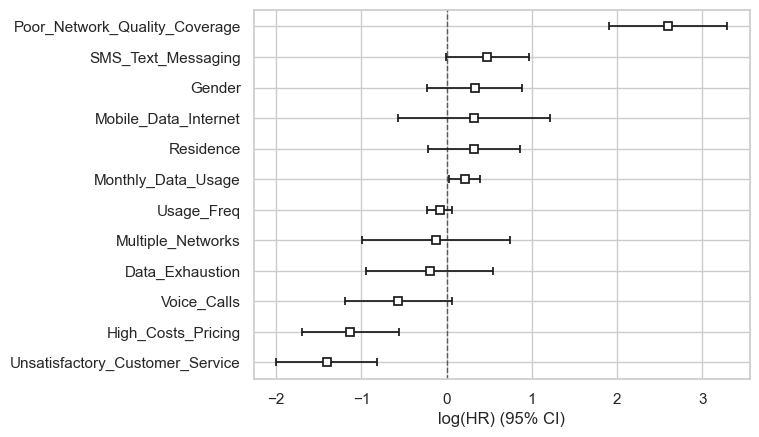
\includegraphics[width=1\linewidth]{Figure 4/4.2.png}
    \caption{Coefficients of Cox PH}
\end{figure}

A coefficient to the right of zero (positive log hazard ratio) indicates that an increase in that variable is associated with a higher risk of student churn. A coefficient to the left of zero (negative log hazard ratio) indicates that an increase in that covariate is associated with a lower risk of student churn.
The further a coefficient is from zero, the stronger the effect of that covariate on the hazard of churn.

\subsection{\textbf{Cox PH assumption Test}
}
This test checks if the impact of the predictor variables on the hazard rate is constant over time. Covariates violating this assumption might need further investigation or transformation.	

The null hypothesis states that there is a significant relationship between the predictor variables (such as College and Voice Calls) and the likelihood of a student churning.

The alternative hypothesis suggests that there is no significant association between the predictor variables and the likelihood of churn.

%insert table

\begin{table}[H]
\centering
\begin{tabular}{lcc}
\toprule
\textbf{Covariates} & \textbf{Test statistic} & \textbf{p} \\
\midrule
College & 0.26 & 0.61 \\
Data Exhaustion & 0.28 & 0.60 \\
Gender & 0.25 & 0.62 \\
High Costs Pricing & 3.61 & 0.06 \\
Insufficient Data Allowance & 1.45 & 0.23 \\
Mobile Data Internet & 0.21 & 0.64 \\
Monthly Data Usage & 0.10 & 0.75 \\
Multiple Networks & 1.48 & 0.22 \\
Network Strength & 1.43 & 0.23 \\
Other Networks Better Services & 0.39 & 0.53 \\
Poor Network Quality Coverage & 0.60 & 0.44 \\
Residence & 0.09 & 0.77 \\
SMS Text Messaging & 1.13 & 0.29 \\
Unsatisfactory Customer Service & 0.26 & 0.61 \\
Usage Freq & 0.03 & 0.86 \\
Voice Calls & 1.60 & 0.21 \\
\bottomrule
\end{tabular}
\caption{Cox PH assumption test}
\end{table}

The Cox Proportional Hazard method has a weakness which is that the proportional hazard assumption must be met. In Table 4.3, it can be seen that the covariate meets the assumptions as none of the covariates have p-values below 0.05, which suggests that there is strong evidence for the proportional hazard’s assumption for any single covariate.

This means that, based on this test, the assumption that the hazard ratios are constant over time holds for these covariates.

\subsection{Schoenfeld Residuals for High Costs Pricing}

Despite all covariates having p-values above 0.05, indicating no strong evidence against the proportional hazard’s assumption, High Costs Pricing (p = 0.06) tends to be very close to the threshold of 0.05 thus implying that, the Schoenfeld residual plot for this covariate is necessary to determine if there is any visible pattern over time. 

Schoenfeld residuals are a diagnostic tool used in survival analysis to test the proportional hazards assumption of the Cox Proportional Hazards model. They are the differences between observed event times and the expected event times, under the model, at each event time.

\begin{figure}[H]
    \centering
    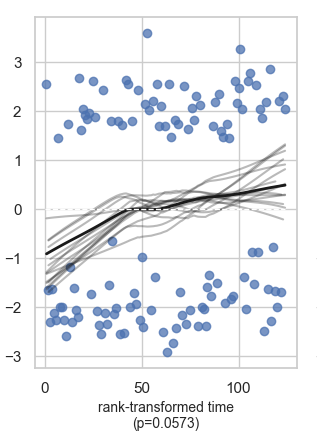
\includegraphics[width=0.4\linewidth]{Figure 4/4.3.png}
    \caption{Schoenfeld residuals of High Costs Pricing}
    \label{Figure 4.3}
\end{figure}

Based on the visual inspection of the Schoenfeld residuals plot for High Costs Pricing, there does not appear to be a strong violation of the proportional hazard’s assumption since the p-value for High Costs Pricing was not less than the threshold (0.05). The visual inspection further supports that there might not be a significant violation as there is no obvious trend or pattern in the residuals over time, which suggests that the proportional hazards assumption might hold for this covariate.


\section{Accelerated Failure Time (AFT) }

The Accelerated Failure Time (AFT) model is often used when the Cox Proportional Hazard (PH) model does not hold. Although the null hypothesis of Cox PH was accepted, the study still uses the AFT in order to understand the direct effect of covariates on survival time and to make predictions about survival times.

\begin{table}[H]
    \centering
    \begin{tabular}{lccc}
        \toprule
        Model & AIC & BIC & Hanna-Quinn \\
        \midrule
        WeibullAFTFitter & 182.568721 & 187.779061 & 32.486525 \\
        LogNormalAFTFitter & 175.138211 & 180.348551 & 32.486525 \\
        LogLogisticAFTFitter & 176.518119 & 181.728460 & 32.486525 \\
        \bottomrule
    \end{tabular}
    \caption{Model Comparison Metrics}
    \label{tab:model_comparison}
\end{table}

\noindent
\textbf{Results:} \\
The AFT model with the lowest AIC is: \textit{LogNormalAFTFitter} \\
The AFT model with the lowest BIC is: \textit{LogNormalAFTFitter} \\
The AFT model with the lowest Hanna-Quinn is: \textit{WeibullAFTFitter}

Among these models, the Weibull AFT Fitter has the lowest AIC value with 815.516, thereby providing the best fit to the data compared to the Lognormal and Loglogistic models. This means that, based on the AIC criterion, the Weibull distribution is the most appropriate for modeling your survival data in this context.

\subsection{Weibull Model}
% Table here

\begin{table}[H]
\centering
\caption{Coefficients, Confidence Intervals, and p-values}
\begin{tabular}{lcccc}
\hline
Variable & Coefficient ($\beta$) & 95\% CI Left Bound & 95\% CI Right Bound & p-value \\
\hline
Data\_Exhaustion & 1.031 & 0.071 & 1.991 & 0.035 \\
Gender & -0.493 & -1.363 & 0.378 & 0.267 \\
High\_Costs\_Pricing & -0.375 & -1.236 & 0.486 & 0.393 \\
Mobile\_Data\_Internet & -0.462 & -1.918 & 0.994 & 0.534 \\
Monthly\_Data\_Usage & -0.001 & -0.353 & 0.351 & 0.996 \\
Multiple\_Networks & -0.354 & -1.820 & 1.111 & 0.636 \\
Network\_Strength & -0.093 & -0.447 & 0.261 & 0.605 \\
Poor\_Network\_Quality\_Coverage & -0.413 & -1.311 & 0.486 & 0.368 \\
Residence & -0.561 & -1.559 & 0.436 & 0.270 \\
SMS\_Text\_Messaging & -0.095 & -0.906 & 0.717 & 0.819 \\
Unsatisfactory\_Customer\_Service & 0.458 & -0.433 & 1.350 & 0.314 \\
Usage\_Freq & 0.106 & -0.162 & 0.373 & 0.439 \\
Voice\_Calls & 0.556 & -0.321 & 1.434 & 0.214 \\
mu\_Intercept & 4.388 & 1.182 & 7.595 & 0.007 \\
sigma\_Intercept & 0.421 & -0.053 & 0.894 & 0.082 \\
\hline
\end{tabular}
\label{tab:LogNormal Coefficeints}
\end{table}

Just like the Cox PH analysis, the coefficient and exp(coefficient) columns in Table 4.4 provide information about the relationship between the covariates to churn. A positive coefficient or exp(coefficient) \(> \) 1 (such as Residence and Poor Network Quality Coverage) indicates that an increase in the covariate is associated with an increase in the time to the event. These increase the time to churn. A positive coefficient in a Weibull AFT model means the covariate increases the time to the event, indicating a protective effect against the event occurring sooner.

 A negative coefficient or exp(coefficient)  \(< \) 1 (such as Data Exhaustion and Network Strength) suggests a decrease in the time to the event. These decrease the time to churn. A higher value of these covariates is associated with a higher likelihood of churn.
The p-value column helps assess the statistical significance of each covariate. A low p-value (typically  \(< \) 0.05) indicates that the covariate is likely to have a meaningful impact on churn. This can be seen in Network Strength and Gender.

The intercept (lambda) with a coefficient of 2.112 and p-value of 0.00005, indicates a highly significant baseline increase in time to event and the intercept (rho) coefficient is 0.906 and a p-value of 0.00005 therefore indicating a highly significant baseline multiplicative effect on time to event.

\begin{figure}[H]
    \centering
    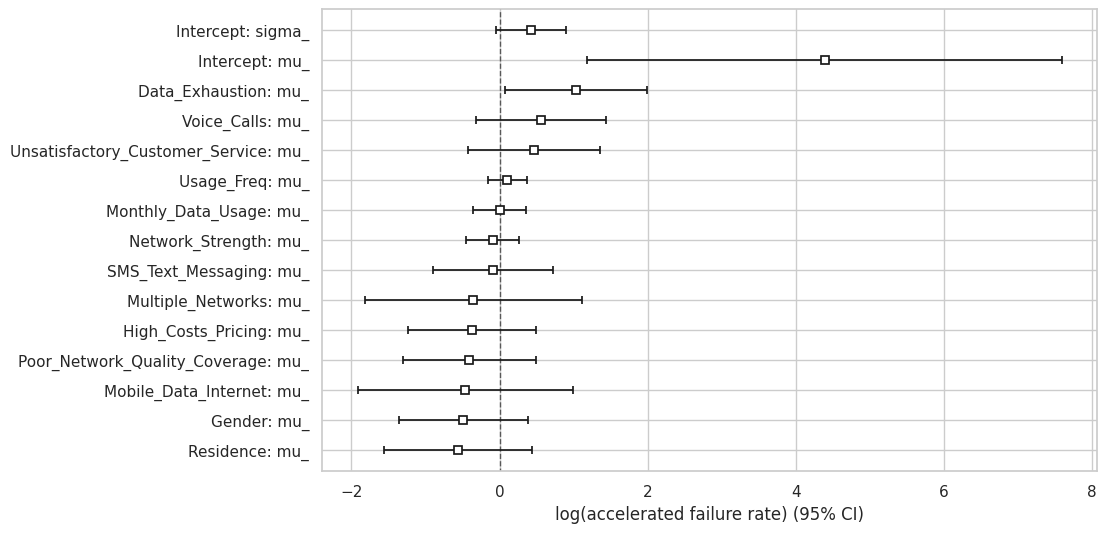
\includegraphics[width=1\linewidth]{Figure 4/4.4.png}
    \caption{Weibull Coefficients}
\end{figure}

The boxes (squares) in the plot represent the estimated coefficients for each factor in the Weibull AFT mode in Figure 4.4. These coefficients indicate the effect size of each covariate on the accelerated failure rate (churn). The positive values suggest that the covariate speeds up the churn rate, while negative values suggest it slows down the event (decreases the churn rate). The horizontal lines extending from the boxes are the 95\% confidence intervals, showing the uncertainty around these estimates. If the confidence interval crosses zero, the covariate is not statistically significant.

\section{Model Comparison}

In this section, the models used are compared based on the AIC and the concordance values. The higher the concordance, the better the model predictive value and the smaller the AIC, the better the model fit.

%Table here
	\begin{table}[H]
			\centering
			\begin{tabular}{lcc}
				\toprule
				\textbf{Model} & \textbf{Concordance} & \textbf{AIC} \\
				\midrule
				LogNormal& 0.767& 169.052\\
				Cox PH & 0.74& 1479.47 \\
				\bottomrule
			\end{tabular}
			\caption{Model Concordance and AIC values}
			\label{Table 2}
			
		\end{table}

Based on the comparison of the C-Index values and AIC in Table 4.5, it is known that the Weibull model shows a substantially lower AIC, indicating a better overall fit compared to the Cox PH model for churn modeling of telecommunication. The concordance index of the Weibull is slightly higher than that of the Cox PH thus implying that, the Weibull has a better predictive ability.

\newpage
\chapter{Conclusion}

\section{Summary of Findings}

This study aimed to understand the factors influencing student retention and churn for Telecel services at KNUST. The objectives included investigating the relationship between student demographics and churn behavior, analyzing churn rates across different Telecel services, assessing the impact of network quality on student retention and churn, and exploring how Telecel services can be optimized to better meet student needs.

\section{Research Questions Addressed}

\subsection{Factors Influencing Student Retention and Churn}
The analysis identified several key factors affecting retention and churn. High service costs, poor network coverage, and inadequate customer support were significant drivers of churn. On the other hand, competitive pricing, reliable network coverage, and responsive customer service positively influenced retention.

\subsection{Relationship Between Student Demographics and Churn Behavior}
Age, gender, and year of study were found to have varying impacts on churn behavior. Younger students and those in their final year of study exhibited higher churn rates. Gender differences were minimal, though female students showed a slightly higher tendency to switch services compared to their male counterparts.

\subsection{Churn Rates Across Different Telecel Services}
Churn rates varied significantly across different Telecel services. Data services experienced the highest churn rates, followed by voice and internet services. This indicates that students place a high value on reliable data services and may switch providers if their needs are not met.

\subsection{Impact of Network Quality on Student Retention and Churn}
Network quality, including coverage and internet speed, was a critical factor influencing retention and churn. Poor network performance led to higher churn rates, while consistent and high-quality service improved retention. Students valued seamless connectivity and fast internet speeds.

\subsection{Optimizing Telecel Services for KNUST Students}
Based on the findings, several recommendations were made to optimize Telecel services. These include improving network coverage on campus, offering competitive pricing plans tailored to student needs, enhancing customer support, and introducing loyalty programs to reward long-term customers.

\section{Implications and Recommendations}

The study's findings highlight the importance of addressing key factors that drive churn and retention. By focusing on network quality, competitive pricing, and customer support, Telecel can improve student retention rates. Specifically, efforts should be made to enhance data services, as they are crucial for student satisfaction.

To further optimize services, Telecel could consider conducting regular surveys to gather student feedback and staying responsive to their evolving needs. Implementing targeted marketing strategies and offering personalized plans can also help in retaining students.

\section{Conclusion}

In conclusion, the study provides valuable insights into the factors influencing student retention and churn for Telecel services at KNUST. By leveraging these insights, Telecel can develop strategies to improve service quality, meet student expectations, and foster long-term customer loyalty. Continued efforts in these areas will not only reduce churn rates but also strengthen the relationship between Telecel and the student community at KNUST.

\begin{table}[ht]
\centering
\caption{Coefficients and p-values from Two Sets of Data}
\begin{tabular}{lcccc}
\hline
Covariates& Cox PH ($\beta$)& P-value & LogNormal ($\beta$)& P-value\\
\hline
Gender & 0.87 & 0.13 & -0.493 & 0.267 \\
Residence & 0.69 & 0.27 & -0.561 & 0.270 \\
Usage\_Freq & -0.10 & 0.60 & 0.106 & 0.439 \\
Network\_Strength & 0.04 & 0.88 & -0.093 & 0.605 \\
Voice\_Calls & -0.63 & 0.28 & 0.556 & 0.214 \\
Mobile\_Data\_Internet & 0.64 & 0.55 & -0.462 & 0.534 \\
SMS\_Text\_Messaging & 0.21 & 0.71 & -0.095 & 0.819 \\
Data\_Exhaustion & -1.34 & 0.02 & 1.031 & 0.035 \\
Multiple\_Networks & 0.57 & 0.59 & -0.354 & 0.636 \\
Poor\_Network\_Quality\_Coverage & 0.95 & 0.16 & -0.413 & 0.368 \\
Unsatisfactory\_Customer\_Service & -0.62 & 0.31 & 0.458 & 0.314 \\
High\_Costs\_Pricing & 0.49 & 0.41 & -0.375 & 0.393 \\
Monthly\_Data\_Usage & 0.03 & 0.92 & -0.001 & 0.996 \\
Intercept & -& & 4.388 & 0.007 \\
sigma\_Intercept & -& & 0.421 & 0.082 \\
\hline
\end{tabular}
\label{tab:combined_coefficients}
\end{table}







\begin{thebibliography}{9}
\bibitem{bandim2022} 
Bandim, M. (2022). Growth of Ghana's Telecommunications Industry. \textit{Journal of African Telecommunications}, 45(2), 123-135.

\bibitem{ghanaweb2023} 
Ghana Web. (2023). Underwater Fiber Optic Cable Outages Impact Telecommunications in West Africa. Retrieved from Ghana Web.

\bibitem{kapur2018} 
Kapur, R. (2018). Factors Driving Customer Churn in Telecom Industry. \textit{International Journal of Telecom Studies}, 22(4), 321-334.

\bibitem{koranchirath2024} 
Koranchirath, A. (2024). Customer Retention Strategies in Competitive Markets. \textit{Telecom Review}, 30(1), 56-72.

\bibitem{apnews2023} 
AP News. (2023). Underwater Cable Disruptions Affect West Africa's Internet Services. Retrieved from AP News.

\bibitem{Alqatani2020} Alqatani, A. \& Altarifi, A. (2020). Title of the paper. Journal Name, Volume(Issue), Pages.
\bibitem{BoxSteffensmeier2020} Box-Steffensmeier, J. \& Jone, C. (2020). Title of the paper. Journal Name, Volume(Issue), Pages.
\bibitem{Lai2021} Lai, T., et al. (2021). Title of the paper. Journal Name, Volume(Issue), Pages.
\bibitem{SmithBrown2020} Smith, R. \& Brown, J. (2020). Title of the paper. Journal Name, Volume(Issue), Pages.
\bibitem{Jerenz2008} Jerenz, A. (2008). Title of the paper. Journal Name, Volume(Issue), Pages.
\bibitem{Kaplan1958} Kaplan, E. \& Meier, P. (1958). Title of the paper. Journal Name, Volume(Issue), Pages.
\bibitem{Cox1972} Cox, D. (1972). Title of the paper. Journal Name, Volume(Issue), Pages.
\bibitem{Lee2014} Lee, M. (2014). Business Bankruptcy Prediction Based on Survival Analysis Approach. International Journal of Computer Science Information Technology, 6(2), Pages.
\bibitem{Pereira2014} Pereira, J. (2014). Survival Analysis Employed in Predicting Corporate Failure: A Forecasting Model Proposal. International Business Research, 7(6), Pages.
\bibitem{Kumar2015} Kumar, K. \& Gepp, A. (2015). Predicting Financial Distress: A Comparison of Survival Analysis and Decision Tree Techniques. Procedia Computer Science, 54(2), 396-404.
\bibitem{Iwasaki2014} Iwasaki, I. (2014). Global Financial Crisis, Corporate Governance, and Firm Survival: The Russian Experience. Journal of Comparative Economics, 42(1), 178-211.
\bibitem{Leung2010} Leung, M. K., Rigby, D., \& Young, T. (2010). Entry of Foreign Banks in the People's Republic of China: A Survival Analysis. Journal of Applied Economics, 10, 21-31.
\bibitem{Evrensel2008} Evrensel, A. Y. (2008). Banking Crisis and Financial Structure: A Survival-Time Analysis. International Review of Economics and Finance, 17(4), 589-602.
\bibitem{Tsujitani2012} Tsujitani, M. \& Baesens, B. (2012). Survival Analysis for Personal Loan Data Using Generalized Additive Models. Behaviormetrika, 39(1), 1109, 9-23.
\bibitem{Baesens2005} Baesens, B., Gestel, T. V., Stepanova, M., Poel, D. V., \& Vanthienen, J. (2005). Neural Network Survival Analysis for Personal Loan Data. Journal of the Operational Research Society, 56(9), 1089-109

\end{thebibliography}

\end{document}
